\documentclass[11pt]{amsbook}
\usepackage{../HBSuerDemir}

\begin{document}
\hPage{b2p2/359}

\begin{hEnumerateArabic}

\item Find the equation of the plane through $(1, 2, 3)$ and making the smallest tetrahedron with the coordinate planes; in the first octant
\\

\item Find the point on $4-z = x^2 + y^2$ which tangent plane at that point makes the smallest tetrahedron with the coordinate planes
\\

\item Find the equation of the line of best fit to data
  \begin{center}
    \begin{tabular}{ c|cccccc }
      x & -1 & 0 & 1 & 2 & 3 & 4 \\
      \hline
      y & 2 & 2 & 4 & 5 & 6 & 8 \\
    \end{tabular}
  \end{center}

\item Find the equation of the parabola of best fit to following data
  \begin{center}
    \begin{tabular}{ c|ccccc }
      x & 0 & 1 & 2 & 3 & 4 \\
      \hline
      y & 3 & 2 & -1 & -6 & -13 \\
    \end{tabular}
  \end{center}
in the form $y = Ax^2 + Bx + C$.

\end{hEnumerateArabic}

\begin{center}
\textbf{ANSWERS TO EVEN NUMBERED EXERCISES}\\
\end{center}

\begin{hEnumerateArabic}

\item[112.]

  \begin{tabular}{p{0pt} p{0.35\textwidth} p{0pt} p{0.35\textwidth}}
    \vspace{0pt} a)
    &
    \vspace{0pt} 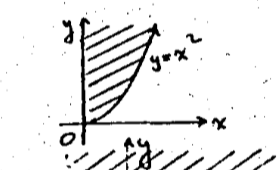
\includegraphics[width=0.35\textwidth]{images/b2p2-359-fig01}
    &
    \vspace{0pt} b)
    &
    \vspace{0pt} 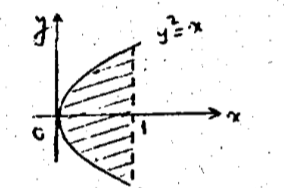
\includegraphics[width=0.35\textwidth]{images/b2p2-359-fig02}
  \end{tabular}
\\

\item[114.]

  \begin{tabular}{p{0pt} p{0.35\textwidth} p{0pt} p{0.35\textwidth}}
    \vspace{0pt} a)
    &
    \vspace{0pt} 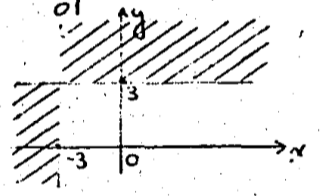
\includegraphics[width=0.35\textwidth]{images/b2p2-359-fig03}
    &
    \vspace{0pt} b)
    &
    \vspace{0pt} 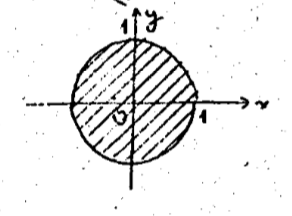
\includegraphics[width=0.35\textwidth]{images/b2p2-359-fig04}
  \end{tabular}
\\

\item[118.]
  \begin{multicols}{2}
    \begin{enumerate}[label={}]
      \item $0$,
      \item $1$
    \end{enumerate}
  \end{multicols}

\item[120.] 2
\\

\item[124.] $ux = (3x^2 + 4)/4u$
\\

\item[128.]
  \begin{multicols}{2}
    \begin{enumerate}[label={}]
      \item $\frac{\partial w}{\partial x} = -\frac{y}{(3x-y)^2}$,
      \item $\frac{\partial w}{\partial y} = \frac{x}{(3x-y)^2}$
    \end{enumerate}
  \end{multicols}

\end{hEnumerateArabic}

\end{document}